% Bar charts
\begin{figure*}[t]
    \centering
    \begin{subfigure}{.3\textwidth}
        \centering
        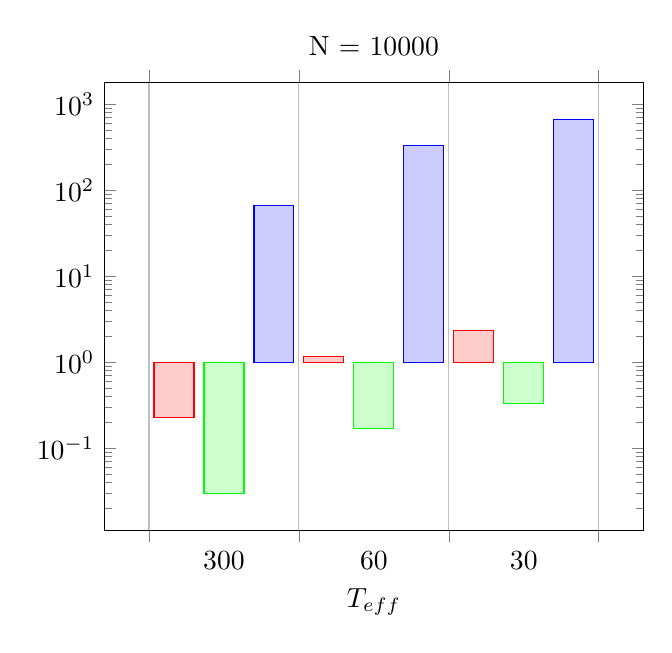
\begin{tikzpicture}
            \begin{axis}[
                title      = {N = 10000},
                enlargelimits=0.1,
                legend pos = outer north east,
                ybar interval = 0.8,
                ymode = log,
                %ylabel={reqs/sec},
                xlabel={\(T_{eff}\)},
                xtick distance = 1,
                symbolic x coords={300,60,30,0},
            ]
            \addplot[
                color=red,
                fill=red!20,
            ]   
                % formula is y = 70 / x
                coordinates {(300,0.23) (60,1.17)
                     (30,2.33) (0,1)};
            %\addlegendentry{S1}
    
            \addplot[
                color=green,
                fill=green!20,
            ]            
            % formula is y = 10 / x
            coordinates {(300,0.03) (60,0.17) 
                    (30,0.33) (0,1)};
            %\addlegendentry{S2}
    
            \addplot[
                color=blue,
                fill=blue!20,
            ]
            % formula is y = 10000 * 2 / x            
            coordinates {(300,66.67) (60,333.33) 
                    (30,666.67) (0,1)};
            %\addlegendentry{Hicks and Garcia}
            \end{axis}
        \end{tikzpicture}
        \caption{Throughput (reqs/sec)}
        \label{fig:eval-reqs}
    \end{subfigure}
    %
    \begin{subfigure}{.3\textwidth}
        \centering
        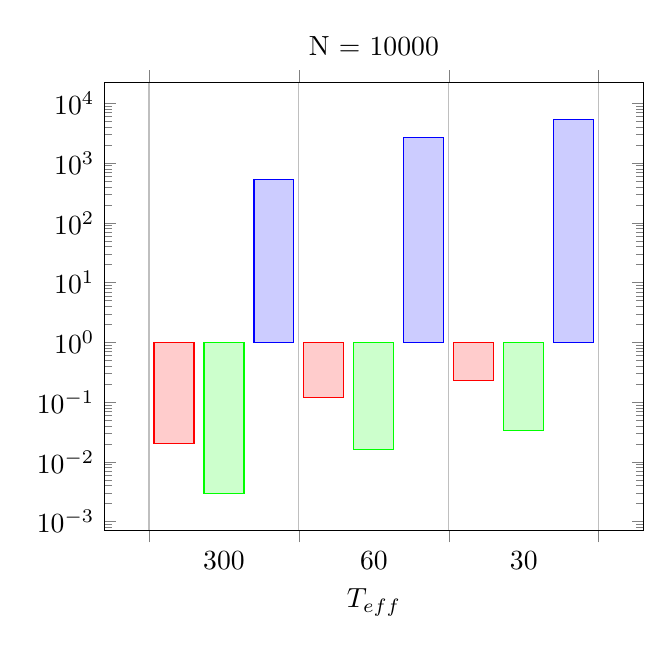
\begin{tikzpicture}
            \begin{axis}[
                title      = {N = 10000},
                enlargelimits=0.1,
                legend pos = outer north east,
                ybar interval = 0.8,
                ymode = log,
                %ylabel     = {CPU (\%)},
                xlabel={\(T_{eff}\)},
                xtick distance = 1,
                symbolic x coords={300,60,30,0},
            ]
            \addplot[
                color=red,
                fill=red!20,
            ]   
                % formula is y = 70 / x * 0.1
                coordinates {(300,0.02) (60,0.12)
                     (30,0.23) (0,1)};
            %\addlegendentry{S1}
    
            \addplot[
                color=green,
                fill=green!20,
            ]            
            % formula is y = 10 / x * 0.1
            coordinates {(300,0.003) (60,0.016) 
                    (30,0.033) (0,1)};
            %\addlegendentry{S2}
    
            \addplot[
                color=blue,
                fill=blue!20,
            ]
            % formula is y = 10000 * 2 / x * 8           
            coordinates {(300,533.33) (60,2666.67) 
                    (30,5333.33) (0,1)};
            %\addlegendentry{Hicks and Garcia}
            \end{axis}
        \end{tikzpicture}
        \caption{CPU usage (\%)}
        \label{fig:eval-cpu}       
    \end{subfigure}
    %
    \begin{subfigure}{.3\textwidth}
        \centering
        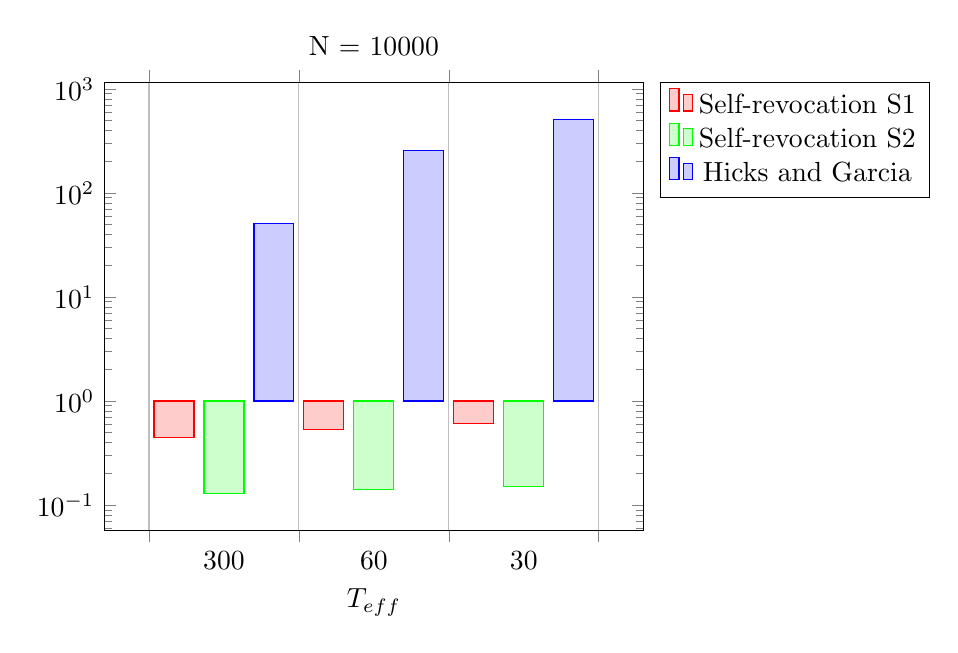
\begin{tikzpicture}
            \begin{axis}[
                title      = {N = 10000},
                enlargelimits=0.1,
                legend pos = outer north east,
                ybar interval = 0.8,
                ymode = log,
                %ylabel     = {CPU (\%)},
                xlabel={\(T_{eff}\)},
                xtick distance = 1,
                symbolic x coords={300,60,30,0},
            ]
            \addplot[
                color=red,
                fill=red!20,
            ]   
            % formula is y = 70 / x * HB_size
            coordinates {(300,0.45) (60,0.53) 
                    (30,0.61) (0,1)};
            \addlegendentry{Self-revocation S1}
    
            \addplot[
                color=green,
                fill=green!20,
            ]            
            % formula is y = 10 / x * HB_size
            coordinates {(300,0.13) (60,0.14) 
                    (30,0.15) (0,1)};
            \addlegendentry{Self-revocation S2}
    
            \addplot[
                color=blue,
                fill=blue!20,
            ]
            % formula is y = 10000 * 2 / x * 780 / 1024          
            coordinates {(300,50.78) (60,253.91) 
                    (30,507.81) (0,1)};
            \addlegendentry{Hicks and Garcia}
            \end{axis}
        \end{tikzpicture}
        \caption{Bandwidth (KB/s)}
        \label{fig:eval-bandwidth}      
    \end{subfigure}
    \caption{Comparison of throughput, CPU usage, and bandwidth between
    self-revocation and short-lived pseudonyms \cite{hicks2020vehicular}, using
    10000 vehicles. The charts show values using $T_{eff}$ equal to 300, 60, and
    30 seconds. The lower the values, the less resources are needed, which
    means the more scalable the protocol is.}
    \label{fig:eval-scalability}  
\end{figure*}